\documentclass[aspectratio=1610,bigger,utf8]{beamer}
\usetheme{Hokie}
\usepackage{graphicx}
\usepackage[scaled]{berasans}
\usepackage[scaled]{beramono}
\usepackage{textcomp}
\usepackage[T1]{fontenc}
\logo{
\includegraphics[height=12pt]{Crystal_Hokie_Tux}}

\title{PGP SUCKS}
\subtitle{a lot\ldots}
\author{Eric C.``echarlie'' Landgraf}
\institute{VTLUUG}
\date{\today}

\begin{document}
\frame{\titlepage}

\begin{frame}
	\frametitle{Contents}
	\tableofcontents[hideallsubsections]

\end{frame}

\section{History}
\subsection{History of PGP}
\begin{frame}
	\frametitle{What Is PGP}
	\begin{itemize}
		\item ``Pretty Good Privacy''
		\item Piece of software and corresponding open standard for
			authenticated and confidential messaging
			\begin{itemize}
				\item Long-lived identity keys
				\item ``Web of Trust'' --- the network of
					people who have verified each others'
					identities.
				\item Strong symmetric and asymmetric
					cryptography
			\end{itemize}
		\item Can be used for local encryption of files, and more often
			for PGP/MIME, that is encrypted and authenticated
			messaging.
	\end{itemize}
\end{frame}
\begin{frame}
	\frametitle{History of ``Pretty Good Privacy''}
	\begin{itemize}
		\item First written by Phil Zimmerman in 1991 with symmetric
			algorithms for anti-nuclear activists. Released
			1991-06-05.
		\item Because it used strong ``weapons-grade'' crypto,
			Zimmerman was investigated by the US Gov't for illegal
			munitions export in early 1993. (PGP used keys >
			40bits)
	\end{itemize}
\end{frame}
\begin{frame}
	\frametitle{History of ``Pretty Good Privacy''}
	\begin{itemize}
		\item PGP 2, later standardized by informational \alert{RFC
			1991} which was published in 1996, was based on RSA; it
			was developed by Viacrypt, who had licence for RSA and
			commercial rights to PGP. PGP 4 was later released by
			Viacrypt as well.
		\item PGP 3 was first released in 1996 and contained DSA and
			ElGamal asymmetric algorithms, as well as CAST-128; all
			were unencumbered by patents. Later released as PGP 5
			in 1997
	\end{itemize}
\end{frame}
\subsection{OpenPGP}
\begin{frame}
	\frametitle{OpenPGP}
	\begin{itemize}
		\item This was formally standardized through the IETF in
			\alert{RFC 2440}, based on the PGP 5 implementation,
			and was published in 1998
		\item Further, this was revised with several later RFCs,
			including \alert{RFC 4880} in 2007
		\item Also notable is the development of PGP/MIME with
			\alert{RFC 2015} and then \alert{RFC 3156} in 1996 and
			2001, respectively
	\end{itemize}
\end{frame}
\begin{frame}
	\frametitle{Versions of PGP}
	\begin{itemize}
		\item PGP 1 --- Completely outdated and irrelevant
		\item PGP 2 --- First PGP incorporating RSA; introduced web of
			trust. Largely supplanted by PGP 5 using stronger
			algorithms.
		\item PGP 3 / PGP 5 (also known as OpenPGP) --- introduced DSA
			and ElGamal keys, which were common for most PGP use
			until the expiration of RSA patents.
		\item GnuPG --- Most common implementation of the OpenPGP
			standard, including libraries for integration into
			other software.
	\end{itemize}
\end{frame}
\section{PGP in theory}
\begin{frame}
	\frametitle{PGP in the Real World}
	\begin{itemize}
		\item If you run a common linux distro, you use PGP
		\item apt, pacman, and yum all rely on PGP to verify package
			integrity
		\item \emph{Most} software developers sign their software
			releases
	\end{itemize}
\end{frame}
\begin{frame}
	\frametitle{What's this ``Web of trust'' thing?}
	\begin{itemize}
		\item Web of Trust (WoT) is a concept pulled from social
			networks (the sociology type, not Facebook).
		\item Basically, human trust models don't reflect machine trust
			models---the WoT bridges this by putting the onus on
			the user to verify identities of others.
		\item No CAs or centralized authorities are relied on.
		\item This has the benefit that you can choose who you trust,
			and how much you trust them, but trust can be
			automatically computed.
	\end{itemize}
\end{frame}
\begin{frame}
	\frametitle{What about keysigning?}
	\begin{itemize}
		\item For the WoT to work, you have to verify identity of other
			users.
		\item This means you hold ``Keysigning parties'' to do just that.
		\item For every key you verify, you're supposed to sign the
			key, and generally put it on public \alert{Keyservers}
			for lookup.
	\end{itemize}
\end{frame}
\begin{frame}
	\frametitle{Modes of operation}
	\begin{itemize}
		\item PGP has 3 modes of operation for asymmetric keys: Signing,
			Encrypting, and Authenticating.
		\item Depending on key algorithm, you need a different type of
			key for each---RSA supports all these modes, but DSA
			does not.
	\end{itemize}
\end{frame}

\section{PGP sucks}
\begin{frame}
	\frametitle{PGP Sucks}
	\begin{itemize}
		\item The standard is complicated---in crypto, this is a bad thing!
			\begin{itemize}
				\item 65 pages for the original standard, RFC 2440
				\item Current draft revision 
					(\alert{RFC 4880bis-02}) is 113
				\item The 5 current standards comprise 130
					pages, and only partially cover what is
					needed to implement PGP
			\end{itemize}
		\item The \alert{tools} are more complicated than the standard!
			GnuPG's primary man page is 71 pages alone, just to
			document the command line flags. And it has texinfo
			documentation, too!
	\end{itemize}
\end{frame}
\subsection{Adobe}
\begin{frame}
	\frametitle{Looks okay, right?}
	\begin{center}
		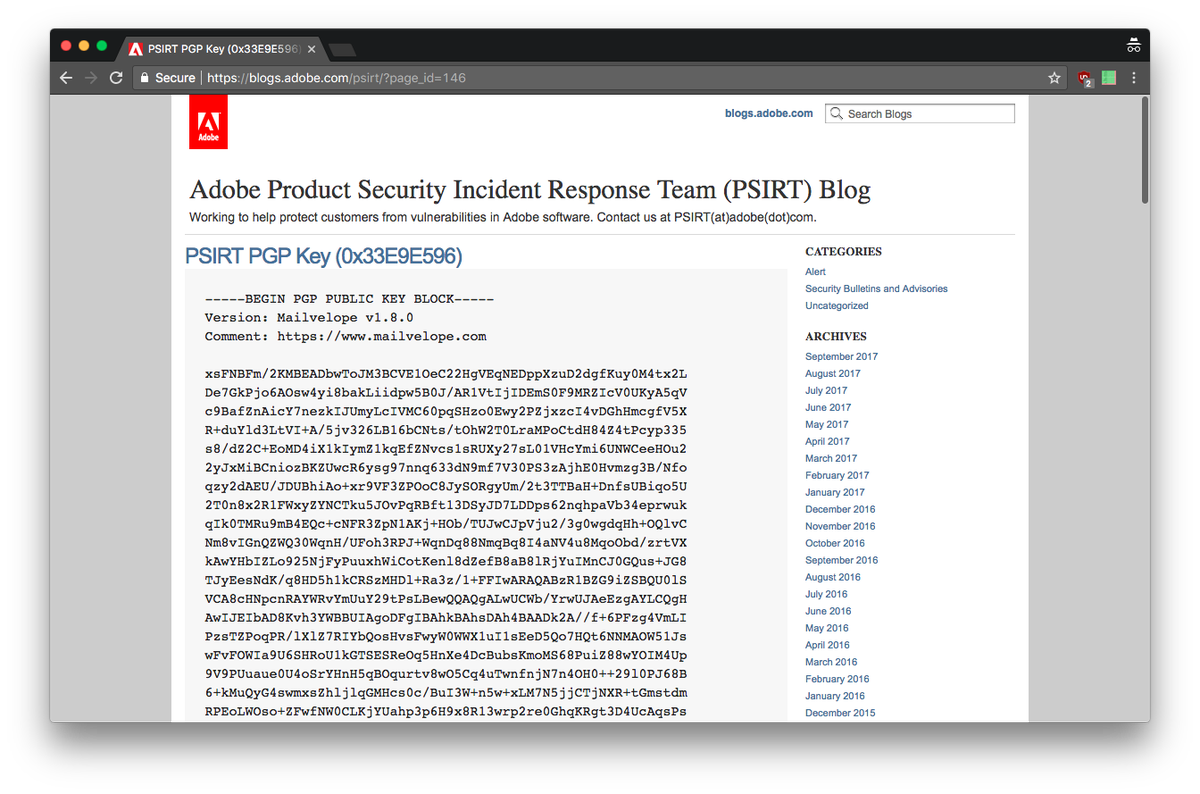
\includegraphics[height=210px]{adobe-1}
	\end{center}
\end{frame}
\begin{frame}
	\frametitle{Hmm\ldots}
	\begin{center}
		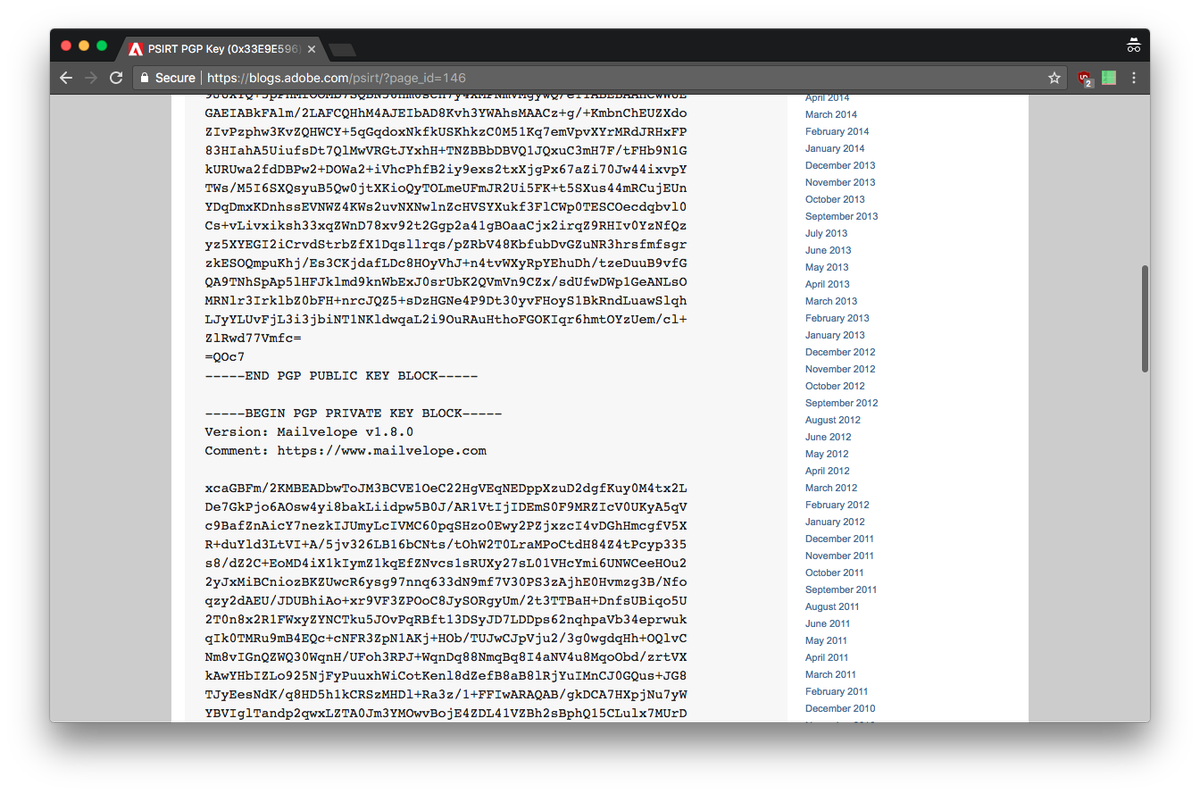
\includegraphics[height=210px]{adobe-2}
	\end{center}
\end{frame}
\begin{frame}
	\frametitle{Well, Shit}
	\begin{center}
		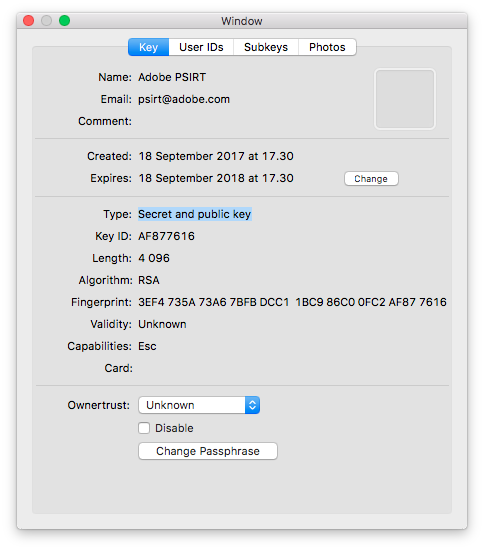
\includegraphics[height=210px]{adobe-3}
	\end{center}
\end{frame}
\subsection{GnuPG}
\begin{frame}
	\frametitle{GnuPG is complicated}
	\begin{itemize}
		\item People fuck this up all the time
		\item Hell; in GPG 2.1, the devs couldn't even write
			dirmngr---one of many components of gpg---to do key
			lookups over IPv6
		\item gpg 2.x have at least 5 different components that have to
			work: dirmngr, gpg-agent, a pinentry program, a
			management tool for gpg-agent, and then the program
			itself.
		\item integration of GPG with smartcards, using it as your ssh
			keyring, and using it for x.509 certificates and s/mime
			all add complexity
	\end{itemize}
\end{frame}
\subsection{Theoretical Flaws}
\begin{frame}
	\frametitle{Key trust is complicated}
	\begin{itemize}
		\item Because of the web of trust, the onus is on you, the
			user, to verify keys with other people.
		\item You have to be \alert{painfully aware of cryptography} to
			understand this---otherwise, verifying identities of
			others, and then \emph{signing keys correctly}, is
			nearly impossible
		\item And then other people have different opinions on
			``sufficient verification''---some verify emails, while
			some only verify identity.
		\item It only approximates human trust models loosely---human
			trust is ephemeral, where PGP trust cannot be.
	\end{itemize}
\end{frame}
\begin{frame}
	\frametitle{Long-lived identity keys suck}
	\begin{itemize}
		\item Ever lose your phone or lose your house keys?\pause\\
			It's kind of \alert{painful} to have to deal with,
			right?\pause
		\item Losing PGP keys sucks so much worse. You potentially
			lock yourself out of everything, and there's no way to
			get it back. If you can't revoke your keys, it's even
			worse---there's no way to validate that you can't use
			your key.\pause
		\item Trust can't be migrated to a new key---if your master key
			uses weak crypto that can be compromised, there's
			nothing you can do about it.
		\item Change your name? Want to use a new algorithm? Time for a
			new key and a complete loss of your trust!
	\end{itemize}
\end{frame}
\subsection{Implementation Flaws}
\begin{frame}
	\frametitle{Implementation Flaws}
	\begin{itemize}
		\item Public keys are \emph{huge} when they have a lot of
			signatures.
		\item The tools don't convey the gravity of actions, and are
			often quite unintuitive.
		\item There are lots of opinions on the \emph{Right
			Way}\texttrademark to use PGP, rather than some
			standard being enforced by the tooling.
		\item Short key IDs are default in most tools; collisions can
			be made.
		\item Trust is largely external to tooling---there aren't many
			good ways to verify people without meeting them
			in-person
	\end{itemize}
\end{frame}
\subsection{Alternatives}
\begin{frame}
	\frametitle{PGP needs to die}
	\begin{itemize}
		\item To be clear, the \alert{crypto} is not the weak part of
			PGP; it's the tooling and the model itself.
		\item better alternatives exist\pause
			\begin{itemize}
				\item signify (openbsd) --- signing only
				\item reop (tedunangst) --- basic encryption only
				\item OTR --- ephemeral message keys and simple trust
				\item signal --- easy-to-use, ephemeral message
					keys, easy-to-establish out-of-band
					trust
				\item plain old s/mime with ca-certs --- better
					supported for email
			\end{itemize}
	\end{itemize}
\end{frame}

\section{Pragmatic PGP}
\begin{frame}
	\frametitle{Pragmatic PGP}
	Still want to use PGP? 
	\begin{itemize}
		\item you're insane, but fine
	\end{itemize}
\end{frame}

\subsection{PGP Trust}
\begin{frame}
	\frametitle{Trust models}
	\begin{itemize}
		\item Most useful feature of PGP is its sense of ``trust'', if
			you're willing to understand it.
			\begin{itemize}
				\item \alert{Note:} trust is often used
					interchangeably with ``authenticity''.
			\end{itemize}
		\item Download a key off a keyserver and look at it; PGP will
			say whether it is trusted or not; this is configurable.
			\begin{itemize}
				\item TOFU
				\item pgp (web of trust)
				\item direct
			\end{itemize}
	\end{itemize}
\end{frame}
\begin{frame}
	\frametitle{Key Validity}
	\begin{itemize}
		\item How can you tell if a key is valid?\pause
		\item Trivial case: unexpired key that you've signed
		\item Or an expired or revoked key---clearly you \emph{shouldn't} trust it\pause
		\item Less trivial: key is signed by people you ``trust''
	\end{itemize}
\end{frame}
\begin{frame}
	\frametitle{Establishing trust}
	\begin{itemize}
		\item Establishing trust is hard, because \alert{trust is
			hard}. PGP simplifies it. ``Your identity has been
			validated by someone I `trust' to verify identities''.
		\item In-person, a glance at hard-to-forge identification may
			do, but what about online?
		\item PGP takes a lot of implicit trust and forces you to make
			it explicit, for it to work.
		\item Some tools, like \url{https://keybase.io} help establish online,
			\alert{persona-based authenticity}.
	\end{itemize}
\end{frame}

\subsection{Threat models}
\begin{frame}
	\frametitle{Threat models}
	\begin{itemize}
		\item PGP does not defend you against all known attacks! The
			\alert{crypto is secure}, but only if you know what it
			does!
		\item Your data and PGP key are \alert{encrypted at rest},
			which is great unless someone installs a
			\alert{keylogger}.
		\item \alert{pew} has copies of my (encrypted) PGP
			subkeys---should I revoke?
	\end{itemize}
\end{frame}
\begin{frame}
	\frametitle{Threat models}
	\begin{itemize}
		\item Expiring and revoking keys help manage threats and trust
		\item If my key is compromised, I can revoke it; if I lose it,
			I can revoke or wait for it to expire
		\item On the other hand, I lose what trust I have---would I
			rather trust an expired key with strong signatures and
			a long life, or a newly generated one?
	\end{itemize}
\end{frame}
\begin{frame}
	\frametitle{Threat models}
	\begin{itemize}
		\item \alert{PGP IS NOT A PANACEA!!!}
		\item If I haven't made it clear, PGP is powerful, but only if
			you understand basic opsec, and what the tool does.
		\item PGP is useless unless you and the party you're communicating with:
			\begin{itemize}
				\item Have PGP keys
				\item Have a ``Secure'' or ``Trusted'' channel
					to establish communications and verify
					each others' identity and key
				\item Can use the tools available.
			\end{itemize}
		\item Sophisticated enemies will \emph{not} target the crypto;
			they'll target the machines you use, the network, or
			the people around you.
	\end{itemize}
\end{frame}
\begin{frame}
	\frametitle{When things fall apart}
	\begin{itemize}
		\item PGP on mobile sucks.
		\item PGP with webmail sucks.
		\item PGP with large non-text files sucks.
		\item PGP provides no anonymity: it is designed for the
			opposite!
		\item PGP provides no forward secrecy: if your encryption
			private key is compromised, all of your encrypted data
			using that key is readable.

	\end{itemize}
\end{frame}

\section{Practical PGP}
\begin{frame}
	\frametitle{Actually using it}
	You'll need an implementation of the OpenPGP tools:
	\begin{itemize}
		\item GNU Privacy Guard (gnupg or GPG) is most common; *nix and
			windows distributions are available
			\begin{itemize}
				\item \url{https://gpgtools.org/} is available
					for OS X
				\item \url{https://www.gpg4win.org/} is a port
					of GnuPG to windows
			\end{itemize}
		\item I have no experience with GPG4Win, or any non-GPG tools;
			many of them provide GUIs, though.
		\item If you're a masochist, I suppose you could use
			\alert{Symantec PGP}. Tell me how that goes.
	\end{itemize}
	I strictly use GnuPG 2.x; 1.4 (shipped by default with Ubuntu and
	Fedora) has a lot of flaws and is not actively developed. Use the
	\texttt{gpg2} binary on these distros.
\end{frame}
\begin{frame}
	\frametitle{A note on PGP GUIs}
	There are a lot of PGP GUIs; both gpgtools and gpg4win ship them. GNOME
	and KDE also have their own. These do not make it much easier to manage
	your key, and make fucking up much easier!

	GNOME Keyring actively sucks when using GPG and \emph{will} get in the
	way eventually!
\end{frame}

\begin{frame}
	\frametitle{Demo}
	Here's where I switch over to a terminal and generate a key, then do
	some things with it. I'll also talk about the ``Perfect'' PGP key.
\end{frame}
\subsection{Keeping your key secure}
\begin{frame}
	\frametitle{Keeping your key secure}
	\begin{itemize}
		\item The security of your key is paramount to PGP's
			effectiveness!
		\item You should obviously use a strong password for your key,
			but there is a lot more you can do:
			\begin{itemize}
				\item back up your key onto an \emph{encrypted}
					drive stored somewhere safe. Check it
					regularly.
				\item strip out your creation key from your
					keyring on devices
				\item print out a copy of your revocation
					certificate; you can OCR it later.
				\item put your key on a yubikey for use on
					``insecure'' machines
			\end{itemize}
	\end{itemize}
\end{frame}

\subsection{Tools to use it with}
\begin{frame}
	\frametitle{Email tools}
	\begin{itemize}
		\item mutt has built-in support
		\item thunderbird through enigmail
		\item mail.app on OS X through a plugin in gpgtools
	\end{itemize}
\end{frame}
\begin{frame}
	\frametitle{password management}
	\begin{itemize}
		\item pass \url{https://www.passwordstore.org/}
			\begin{itemize}
				\item pass has numerous wrappers and plugins
					for use on non-unix platforms
				\item use of asymmetric crypto is also a boon
					when using with teams
			\end{itemize}
		\item Implementing your own is pretty easy (there are plenty of
			people who do)
	\end{itemize}
\end{frame}
\begin{frame}
	\frametitle{SSH}
	It's also possible to use your gpg-agent as an ssh agent, and a gpg key
	as an ssh key. This works really nicely with a yubikey and shared
	workstations!
\end{frame}
 
\end{document}
